\section{Введение}
В современное время в кардиологии начинается активное использование поверхностное ЭКГ-картирования. 
Данное понятие представляет собой одномоментную регистрацию множественных отведений ЭКГ со всей поверхности грудной клетки.
Это исследование, основанное на распределении электрических потенциалов сердца на поверхность грудной клетки.
Данная методика направлена на изучение нормальной и патологической электрофизиологии сердца.
При использовании привычной всем стандартной ЭКГ, все до этого перенесенные инфарткты миокарда, эктопические комплексы,
синдромы предвозбуждения желудочков создают условия, которые препятствуют качественной классификации и диагностики электрофизиологических параметров.
В отличие от общепринятых методик электрокардиографии, в которых измеряются и анализируются параметры
электрического поля сердца в небольшом числе точек поверхности торса, в методах картирования применяются множественные датчики, 
а сигналы от всех этих датчиков регистрируются синхронно, что позволяет изучать характеристики и параметров ЭКГ, 
даже при документированных сердечных аномалиях. Получаемые результаты в определенный промежуток времени
будут представляться в виде цветовой диаграммы в определенный промежуток времени.

По характеристикам поверхностного ЭКГ-картирования можно оценить
следующие параметры: характер распределения потенциалов (дипольность-
мультипольность), расположение экстремумов потенциалов, величина
экстремумов, наличие нетипичных положительных и отрицательных зон,
направление и скорость движения фронтов возбуждения.

Примеры изопотенциальных карт приведены на рис. 1. Схематическая
развертка грудной клетки представлена как цилиндрическая поверхность,
разомкнутая по правой задне-подмышечной линии. Для построения карты (в
указанный момент времени сердечного цикла) точки, имеющие равный
потенциал, соединяются линиями. Точки, имеющие положительный
потенциал, создают позитивную зону (незакрашенная область) с
максимумом потенциала («+», числовое значение приведено в мкВ), а точки,
имеющие отрицательный потенциал, создают негативную зону (закрашенная
область) с минимумом потенциала («-», числовое значение приведено в
мкВ).



\begin{figure}[ht!]
\begin{center}
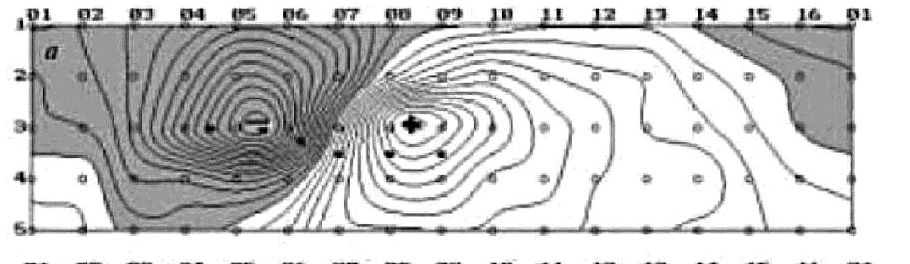
\includegraphics[scale=0.5]{ris1}
\end{center}
\caption{Типичное распределение потенциалов на изопотенциальных картах процесса депоряризации и реполяризации желудочков}\label{ris1}
\end{figure}

Имея такую модель, медицинские работки смогут более наглядно
получать данные и сопоставлять их с реальными физическими процессами.
Для обеспечения их необходимой поддержкой будет создан
интегрированный аппаратно-программный комплекс.


Программный комлекс будет представлять собой интерфейс, состоящий из окошка, в котором данные исследования будут представлены 
в виде цветовой диаграммы. В отличие от стандартного ЭКГ, где используется 13 датчиков, в поверхностном ЭКГ-картировании
используется 80 датчиков. 5 рядов по 16. Каждый из 80 значений будет являться числом, которое будет иметь определенный цвет в шкале.
\begin{figure}[ht!]
\begin{center}
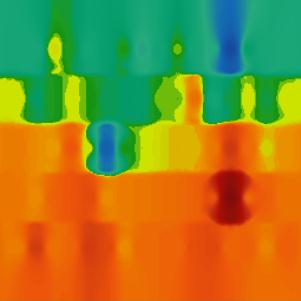
\includegraphics[scale=0.85]{ris2}
\end{center}
\caption{Пример цветовой диаграммы}\label{ris2}
\end{figure}

Так будет выглядеть результат обследования. 
Так же в окошке приложения будет расшифрофка цветовой шкалы и бегунок, который позволит просмотреть результат в определеный промежуток времени.



Второй частью выполнения работы будет разработка программного комплекса для анализа данных поверхностного
ЭКГ-картирования при помощи многослойного персептрона. Данный комплекс будет создаваться с целью выявления у людей, страдающих ожирением, скрытой эшемии
на основе анализа данных, взятых при помощи поверхностного ЭКГ-картирования на
аппарате Astrocard. 





